\addcontentsline{toc}{section}{Anhang}
\section*{Anhang}
\appendix

\addtocontents{toc}{\protect\setcounter{tocdepth}{2}}
\makeatletter
\addtocontents{toc}{%
  \begingroup
  \let\protect\l@section\protect\l@subsection
  \let\protect\l@subsection\protect\l@subsubsection
}
\makeatother

\section{Mikroinstruktionen und Speicherzugriffe}
\label{appendix:microinstructions}
Mikroinstruktionen sind eine minimale Reihe an in Hardware
in der \ac{CPU} implementierten Befehlen zum Ausführen von
Operationen. Die Komplexität und Menge
dieser Instruktionen werden bewusst möglichst gering gehalten,
um das Design der Hardware zu vereinfachen. Sie
beschreiben die konkreten Hardwareschritte, um komplexere
Befehle der \ac{ISA} auszuführen. Sie haben außerdem keinen
Speicherzugriff, sondern implementierten lediglich die
Interaktion mit der Hardware der Speicherkomponenten.
Auch wenn diese Abstraktion zu einem entsprechenden
Performanceverlust aufgrund der Übersetzung von
\ac{ISA}-Instruktionen führt, sind moderne \acp{CPU}
mikrocodebasiert, da dies das Updaten von komplexeren
Instruktionen bei Bugs oder Performanceproblemen in der \ac{ISA}
ermöglicht. Die Anwendung entsprechender Patches für das
Verhindern von Cache-basierten Covert-Channels und Angriffen
mit spekulativer Ausführung ist nur begrenzt möglich, da es
sich bei diesen Angriffsvektoren um logische und konzeptionelle
Eigenschaften handelt, die ausgenutzt werden.
(\cite[380,386,395]{sarangi_basic_2021})
Instruktionen werden in derselben Reihenfolge in
Mikroinstruktionen übersetzt, wie sie in die Pipeline geladen
werden. Eine Branch-Prediction, um Instruktionen zu prefetchen,
ist also nicht nötig.
Dennoch existiert Logik, um das Ergebnis von Branch
Instruktionen in Mikrocode vorherzusagen. \cite[6,7]{mosier_analyzing_2025}
zufolge kann dieser Predictor auch für \acp{TEA} ausgenutzt werden
und ist für Ursache für verschiedene bekannte Arten an \acp{TEA}.

\section{Grundlegende Cache Architekturen}
\label{appendix:basic-cache-arch}
Die zwei grundlegendsten Cache-Mapping-Methoden sind der
Fully-Associative und der Direct-Mapped Cache. Bei dem Fully
Associative Cache besteht der physische Adress-Speicher aus einer
Reihe an Speicherzellen, in denen die Adresse des aktuell gespeicherten
Blocks zusammen mit dem entsprechenden Block abgelegt wird.
Hierbei sei angemerkt, dass die Blockadresse einfach als die
ersten $N$ Bits der physischen Adresse realisiert werden kann.
Dadurch, dass eine Adresse in jedem Eintrag gespeichert werden kann,
kann durch eine Cache-Policy immer dafür gesorgt werden, dass
die meistgenutzten Blöcke im Cache bleiben. Das bedeutet, wenn
eine Adresse in den Cache geladen wird und der Cache ist bereits
voll, wird anhand der Cache-Policy entschieden, welcher Eintrag
ersetzt wird. Dafür muss allerdings bei einem Cache-Zugriff
über sehr viele Einträge iteriert werden, was zu einem
deutlichen Zeitaufwand führt.

Bei einem Direct-Mapped-Cache dagegen hat jeder Block einen
eindeutigen Cache-Eintrag, in dem er gespeichert werden kann.
Dafür können zum Beispiel die letzten $N$ Bit einer Adresse
verwendet werden, wobei $N$ die Länge der binären Blockadresse
ist. Der Vorteil ist hier, dass beim Laden eines Blocks sofort
klar ist, welcher Eintrag ersetzt werden muss. Der Nachteil ist,
dass sehr häufig viel genutzte Adressen um denselben Cache-Eintrag
konkurrieren, was große Verzögerungen bei Speicherzugriffen
zur Folge hat.
(\cite[518-521]{sarangi_basic_2021}, \cite[16-18]{handy_cache_1993})

Aus diesem Grund wird eine Kombination der beiden
Mapping-Methoden, ein \ac{SAC}, verwendet. Dabei wird jede Adresse
mit einer Menge an Einträgen assoziiert. Die Adresse dieses Sets
hat eine Länge von $N = B - a$, wobei B die Länge der Blockadresse
und $a$ die Assoziativität des Cache ist, welche die
Größe der Sets bestimmt (Größe der Sets $s=2^a$). Der Vorteil
ist, dass konkurrierende und miteinander assoziierte Adressen,
zumindest bis zu einem gewissen Punkt, gleichzeitig in dem Cache
bleiben können. Dafür muss allerdings eine Cache-Policy für jedes
Set und damit auch gewisse Zugriffsinformationen implementiert
werden. Durch die limitierte Größe des Cache-Sets muss allerdings
dafür nicht durch zu viele Einträge iteriert werden.
(\cite[522-524]{sarangi_basic_2021}, \cite[18,19]{handy_cache_1993})

\section{Mehrschichtiger Cache}
\label{appendix:multilayer-cache}
Mehrere Cache-Layer sind nötig, da mit zunehmender Cache-Größe
die Zugriffszeit steigt.
Zusätzlich werden private Caches für Kerne implementiert, um die
Datenraten bei Cachezugriffen nicht zwischen den Kernen
aufzuteilen.
(\cite[388]{slomka_grundlagen_2023}, \cite[593]{sarangi_basic_2021})

Durch die mehrschichtige Architektur muss außerdem sichergestellt
werden, dass Schreiboperationen auch in den darauffolgenden
Schichten persistiert werden. Dazu gibt es das „write-trough“
Prinzip, bei dem jede Schreiboperation direkt eine
Schreiboperation in den folgenden Schichte auslöst, und das
„write-back“ Prinzip, bei dem eine Schreiboperation den Block
mit einem Bit als modifiziert markiert und bei dem Entfernen
des Blocks aus dem Cache eine Schreiboperation aufruft.
(\cite[526]{sarangi_basic_2021})

Bei inclusive Cache-Layern muss zudem sichergestellt werden,
dass eine Eviction auf allen Cache-Layern stattfindet. Bei dem
Aufruf einer \verb|clflush|-Instruktion kann die Ausführung
früher fortgeführt werden, wenn sich die Adresse nicht im
\ac{LLC} befindet. Es reicht, den \ac{LLC} anzusteuern und bei
einem Cache Miss die Ausführung fortzusetzen. Bei einem Hit muss
der Block aus dem Cache geflusht und ein Flush-Befehl an alle
weiteren Cache-Layer gesendet werden. Daher folgt ein zeitlicher
Unterschied bei der \verb|clflush|-Instruktion, wenn die Adresse
gecacht ist. (\cite[4]{caballero_flushflush_2016})

\section{Spekulative Ausführung von Branch Instruktionen}
\label{appendix:speculative-branches}
Wie bereits erwähnt wird für pipelined Prozessoren ein
Prefetching-Mechanismus implementiert, um die Abhängigkeit der
Auslastung der Pipeline von der Speichergeschwindigkeit zu
verringern. Bei Branch-Instruktionen kann sich allerdings
die Folge-Instruktion ändern und damit der Control-Flow verändert
werden. Das Problem ist, dass die Entscheidung, ob der Branch
genommen wird und welchen Wert demnach der \ac{PC} annimmt, erst
in der Pipeline entschieden wird und zusätzlich von Werten im
Speicher abhängig sein kann.
(\cite[14,15,40]{kaeli_speculative_2005})

Um dennoch die Pipeline auszulasten, werden verschiedene
Mechanismen verwendet, um Folgeinstruktionen auszuführen. Das
Prefetching ist primär davon abhängig, ob ein Branch genommen
wird oder nicht. Dabei ist zu beachten, dass sich das Prefetching
zeitlich vor der Pipeline befindet, bei einer Branch-Instruktion
allerdings die direkt darauf folgende Instruktion abhängig von der
Entscheidung ist. Die Vorhersage und damit auch die Änderung der
nächsten Instruktionen, die vom Prefetcher geladen werden, kann
an verschiedenen Stellen, mit verschiedenen Vor- und Nachteilen,
dieser Architektur stattfinden. Je früher die Vorhersage
stattfindet, desto weniger Informationen sind zu der
Instruktion bekannt, und folglich verschlechtert sich die
Genauigkeit der Vorhersage. Je später allerdings die Entscheidung
getroffen wird, desto mehr Instruktionen wurden bereits transient
in der Pipeline ausgeführt und müssen verworfen werden. Neben der
Betrachtung, ob der Branch genommen wird, muss auch das Ziel
bestimmt werden, um die korrekten Instruktionen zu laden. Je
nachdem, ob die Zieladresse ein Literal oder ein dynamischer Wert
ist, kann dies eine Abhängigkeit sein, von deren Auflösung
abhängt, wie weit die Pipeline fortgeschritten ist. Mit der
Entscheidung, ob der Branch genommen wird und was das Ziel ist,
wird nicht nur das Ziel des Prefetchers geändert, sondern auch
die entsprechenden Instruktionen bis zur Auflösung des Branches
werden ausgeführt. Ob ein Branch genommen wird oder nicht, kann
statisch z.B. anhand der konkreten Instruktion, oder dynamisch
z.B. anhand vergangener Branch-Entscheidungen entschieden werden.
Da bei einer Branch-Entscheidung nur einer der zwei Pfade weiter
ausgeführt wird, wird diese Art von spekulativer Ausführung auch
„unipath“ Execution genannt.
(\cite[40,42-48,136]{kaeli_speculative_2005})

Dem gegenüber steht die „multipath“-Execution. Dabei werden beide
Pfade ausgeführt und wenn die Branch-Entscheidung getroffen wird,
werden die falsch ausgeführten Instruktionen verworfen. In
einer \ac{CPU}-Architektur können außerdem auch beide Konzepte
implementiert werden. Dabei kann ein Predictor verwendet werden,
der auch eine Konfidenz seiner Vorhersage angibt, und bei geringer
Konfidenz können beide Pfade ausgeführt werden. Der Vorteil von
Multipath-Execution ist, dass die Pipeline voll ausgelastet
werden kann und die Ergebnisse nicht vollständig verworfen
werden. Der Nachteil gegenüber unipath Execution ist wiederum,
dass 2 Pfade ausgeführt werden und dies eine zusätzliche
\ac{CPU}-Last darstellt. Besonders bei mehreren nicht aufgelösten
Branch-Entscheidungen sammeln sich diese Pfade.
(\cite[136,137]{kaeli_speculative_2005})

\section{Weitere technische Möglichkeiten für Covert-Channel in
der Prozessorarchitektur}
\label{appendix:advanced-cbcc}
Viele Covert-Channel Übertragungen basieren darauf, dass die Nutzung
von geteilten Ressourcen von dem Sender so ausgenutzt wird, dass
diese Nutzung für den Empfänger messbar wird. Ein Beispiel für
die Nutzung von geteilten Ressourcen ist die Cache-Bandbreite,
das heißt die Menge an load-Instruktionen, die von der
Speicher-Architektur in einer gewissen Zeit beantwortet wird.
\cite{wang_bandwidthbreach_2023} nutzen beispielsweise den
\ac{LFB}, der Speicherzugriffe speichert, die den L1 Cache
verfehlen, aus, um die Bandbreite von Cache-Zugriffen zu
begrenzen. Dabei werden vom Sender konkret um eine logische 1 zu
übertragen Instruktionen wie „vmovntdq“ ausgeführt, die lange
im \ac{LFB} bleiben und damit die Ausführung von Speicherzugriffen
des Empfängers in derselben Pipeline verzögern. Dafür
müssen die Prozesse von Sender und Empfänger zur gleichen Zeit
auf dem gleichen physischen Kern ausgeführt werden, was ein
Feature wie \ac{SMT} voraussetzt. Außerdem kann dieser
Covert-Channel nicht im Kontext von Transient Execution genutzt
werden, da das Schreiben und Lesen dafür sequenziell ausgeführt
werden müssen. Ein ähnlicher Covert-Channel ohne die Verwendung
von Cache-Ressourcen wird in \cite[2]{wang_covert_2006} vorgestellt.
In diesem Falle werden Informationen in Form der Belegung
bestimmter geteilter Recheneinheiten in demselben physischen Kern
enkodiert. Durch das Ausführen vieler
Multiplikations-Instruktionen kann die Pipeline eines Empfängers
in demselben physischen Kern verzögert werden, wenn dieser auch
Multiplikations-Instruktionen ausführt.
Ein weiteres Beispiel wird in \cite[9,10]{paccagnella_lord_2021}
demonstriert. Dort wird der zentrale Bus der \ac{CPU} für die
Kommunikation mit dem \ac{LLC} für contention verwendet, wodurch
dieser Covert-Channel auch für cross-core Kommunikation verwendet
werden kann.

Da alle dieser Covert-Channel contentionbasiert sind, sind sie
nur bedingt für den Kontext von Transient Execution anwendbar.

\section{Erläuterung zu verschiedenen \ac{CbCC} Techniken}
\label{appendix:cbcc-techniques}
Zum Zeitpunkt der Veröffentlichung von
\citetitle{kocher_spectre_2019} existierte bereits eine Menge
Literatur zu cachebasierten Side-Channels, die praktisch genauso
auch als \ac{CbCC} verwendet werden konnten. Noch heute wird in
vielen \acp{TEA} in der Literatur
Side-Channel Techniken wie Flush+Reload
(\cite{yarom_flushreload_2014}) verwendet
(\cite[7]{schwarz_zombieload_2019}, \cite[91]{van_schaik_ridl_2019},
\cite[6]{kim_flop_2025}, \cite[6]{kim_slap_2025},
\cite[3]{hertogh_rain_nodate}).

Andere \ac{CbCC}, die höhere Bandbreiten durch geringere
Zugriffszeiten der unteren Cache-Layer ausnutzen, sind meistens
an gewisse Bedingungen geknüpft, wie die Ausführung beider Kontexte
auf demselben Kern. Ein Beispiel dafür sind Demote+Reload und
Demote+Demote, welche die \verb|cldemote|-Instruktion
(\cite{noauthor_cldemote_2023}) nutzen, um Cache-Lines aus dem
L1 Cache zu evicten und in den L2 bis \ac{LLC} Cache zu verschieben.
Diese Instruktion wurde allerdings erst in neueren
Intel-\ac{CPU}-Generationen zur \ac{ISA} hinzugefügt, und ist damit
nicht in jeder x86-\ac{CPU} verfügbar (\cite{noauthor_list_2026}).
Der große Vorteil von \verb|cldemote| ist, dass keine Speicherzugriffe
und keine Operationen über den \ac{LLC} hinaus nötig sind.
Zusätzlich implementieren neuere \acp{CPU} non-inclusive \acp{LLC},
was bisherige cross-core \ac{CbCC} komplizierter macht, da
Interaktionen des Zielkontexts, auf einem anderen \ac{CPU}-Kern
und in dessen private Caches, keine Veränderung in dem \ac{LLC}
zur Folge haben müssen. (\cite[3,4]{rauscher_systematic_2025})

Auch für \acp{CPU} mit inclusive \ac{LLC} und ohne \verb|cldemote|
wurde schon deutlich früher ein ähnlicher evictionbasierter
\ac{CbCC} demonstriert. Bei \cite[6,7]{almgren_c5_2015} lädt der
Angreifer eine Adresse in den \ac{LLC}, die aufgrund von starker
Cacheauslastung evicted wird. Diese Cacheauslastung wird von dem
Zielkontext ausgelöst, indem viele Adressen geschrieben und damit
in allen Cache-Layern gesetzt werden. Werden keine Werte
geschrieben, dann wird die Adresse des Angreifers nicht evicted,
was für den Angreifer messbar ist. Dieser Covert-Channel wurde
allerdings nicht in dem Kontext von Transient Execution evaluiert
und ist in diesem Kontext wahrscheinlich aufgrund der Anzahl an
Schreibinstruktionen technisch nicht umsetzbar.

\section{Erläuterung zu der Messung, ob eine Adresse gecacht ist}
\label{appendix:explanation-on-cache-measurements}
Eine Grenze, mit der bestimmt wird, ob eine
Adresse gecacht ist oder nicht, kann praktisch nur statistisch
ermittelt werden. Diese Grenze hat erheblichen Einfluss auf die
Genauigkeit des \ac{CbCC}, da sie die Metrik definiert, ob ein
korrekt encodierter Wert auch korrekt ausgelesen wird.
Vergangene Messungen zu Cache-basierten Side-Channels
(\cite[6,7]{yarom_flushreload_2014}, \cite[5-7]{rauscher_systematic_2025})
zeigen, dass der zeitliche Unterschied zwischen den zwei
betrachteten Zuständen klar unterscheidbar ist. Allerdings kann
je nach Software, Hardwareumgebung und Systemauslastung
die Dauer solcher Zugriffe deutlich variieren
(\cite[7]{yarom_flushreload_2014}). Aus diesem Grund wurde diese
Grenze auch häufig manuell bestimmt. Um \ac{CbCC} allerdings für
verschiedene Konfigurationen nutzbar zu machen, wird
in dem Test-Programm dynamisch vor der Übertragung eine
Grenze ermittelt. Diese Strategie zur Ermittlung der Grenze wird in
dieser Arbeit konzeptionell nicht tiefer evaluiert, sondern nur
beschrieben.

Die Grenze wird auf Basis von 100 Messungen von Adressen,
die vorher geladen wurden, und 100 Messungen, die vorher
geflusht wurden, berechnet. Diese Adressen werden als Array
allokiert. Um die Unabhängigkeit dieser Adressen sicherzustellen
und ein Prefetching zu verhindern, wird jede Messung mit Index $i$
semizufällig mit dem randomisierten Index $r$ durchgeführt, genauso
wie in \cite[19]{kocher_spectre_2019}:
\[r=(i*167)+67\mod 100\]
Dabei sei zu beachten, dass 167 und 67 Primzahlen sind und somit
eine eindeutige Indizierung sicherstellen.
Darüber hinaus wird angenommen, dass die Zugriffszeiten
normalverteilt sind, obwohl Speicherzugriffe aus physischen
Gründen eine untere Grenze haben und, zumindest in virtualisierten
Umgebungen, mit geringer Wahrscheinlichkeit Zugriffe auf den
Speicher sehr hohe Zugriffszeiten haben können
(\cite[7]{yarom_flushreload_2014}). Diese Annahme wird
dennoch getroffen, um die Komplexität zu verringern.

Aus den 100 Messwerten wird jeweils das arithmetische
Mittel für die Laufzeit, der geflushten Adressen $f$,
sowie der geladenen Adressen $c$, gebildet und daraus
folgendermaßen eine Grenze $g$ berechnet:
\[g=c+\left(\frac{f-c}{2}\right)\]

\clearpage
\section{Abbildungen zur theoretischen Laufzeit einer Übertragung bei \acp{TEA}}
\begin{figure}[H]
    \centering
    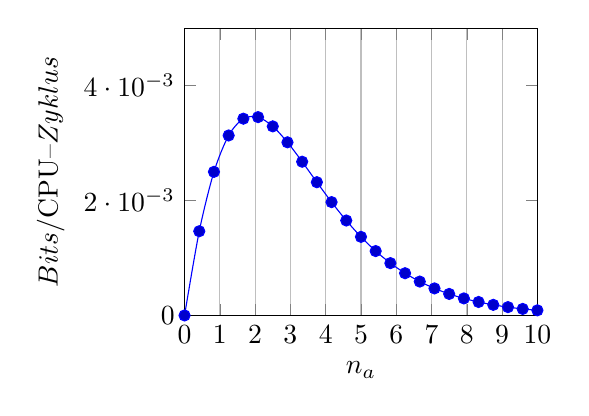
\begin{tikzpicture}
        \begin{axis}[
                width=0.5\textwidth,
                xtick distance=1,
                scaled ticks=false,
                xlabel={$n_a$},
                ylabel={$Bits$/\ac{CPU}\textendash $Zyklus$},
                xmin=0,xmax=10,
                ymin=0,ymax=0.005,
                xmajorgrids,
            ]
            \addplot+ [
                id=runtime,
                smooth,
                domain=0:10,
            ] plot (\x, {(8*\x)/((50*20) + 100 + (8*50*2^(\x)-1) + (8*120*2^(\x-1)))});
        \end{axis}
    \end{tikzpicture}
    \caption{$D(n_a)$ mit $N_T=50$, $T_T=20$, $L_E=100$,
    $T_P=50$, $T_R=120$ und $n_{bmax}=8$\label{figure:theoretical-runtime}}
\end{figure}

\begin{figure}[H]
    \footnotesize
    \[D'(n_a)=-\frac{2n_{bmax} \left(n_{bmax} \left(\left(\ln\left(2\right) \left(T_R + 2T_P\right) n_a - T_R\right) \cdot 2^{n_a} - 2T_P \left(2^{n_a} - 1\right)\right) - 2 \left(N_TT_T + L_E\right)\right)}{\left(n_{bmax} \left(T_R \cdot 2^{n_a} + 2T_P \left(2^{n_a} - 1\right)\right) + 2 \left(N_TT_T + L_E\right)\right)^{2}}\]
    \caption{Die erste Ableitung der Durchsatz-Funktion $D(n_a)$\label{figure:throughput-derivation}}
\end{figure}

\section{Programmausschnitte des Test-Programms}
\begin{lstlisting}[caption={Funktion, die Transient Execution in
    dem Test-Programm auslöst},
    label={listing:transient-function},captionpos=b]
inline __always_inline bool leak_data(void (*asm_encode)(uint64_t data, uint8_t *channel,
                                  uint8_t bits_count, uint64_t stride),
               uint32_t iteration, uint32_t *train_data,
               uint32_t train_data_len, uint64_t secret, uint8_t channel[],
               uint8_t bits_count, uint64_t stride)
{
    if (train_data[iteration] < train_data_len)
    {
        asm_encode(secret, channel, bits_count, stride);
        return true;
    }
    return false;
}
\end{lstlisting}

\begin{lstlisting}[caption={Funktion für die bitweise Encodierung
    eines Secrets in den Covert-Channel},
    label={listing:cbcc-binary-encoding},captionpos=b]
static inline __always_inline void asm_encode_load_bitwise(
    uint64_t data, uint8_t *channel,
    uint8_t bits_count, uint64_t stride)
{
    __asm__ volatile("xor %%rax, %%rax\n"

                     "movb $0x0, %%bl\n"
                     "movq $0x1, %%rcx\n"
                     "movq %[stride], %%rdx\n"
                     "movb %[bitscount], %%sil\n"
                     "enc0:\n"

                     "addb $0x1, %%bl\n"
                     "addq %%rdx,%[channel]\n"
                     "movq %[data], %%rax\n"
                     "andq %%rcx, %%rax\n"
                     "testq %%rax, %%rax\n"
                     "jz nenc0\n"
                     "prefetcht0 (%[channel])\n"

                     "nenc0:\n"
                     "sal $0x1, %%rcx\n"
                     "cmpb %%sil, %%bl\n"
                     "jne enc0\n"
                     :
                     : [data] "r"(data), [channel] "r"(channel), [stride] "r"(stride), [bitscount] "r"(bits_count)
                     : "rax", "rbx", "rcx", "rdx", "rsi", "cc");
}
\end{lstlisting}

\section{Cache Spezifikationen der verwendeten \acp{CPU}}
\label{appendix:lscpu-cache}
\begin{lstlisting}[caption={Ausagbe von lscpu und lscpu --caches des
Intel\textregistered\space Core\texttrademark\space i7-6700K}]
Architecture:                            x86_64
CPU op-mode(s):                          32-bit, 64-bit
Address sizes:                           39 bits physical, 48 bits virtual
Byte Order:                              Little Endian
CPU(s):                                  8
On-line CPU(s) list:                     0-7
Vendor ID:                               GenuineIntel
Model name:                              Intel(R) Core(TM) i7-6700K CPU @ 4.00GHz
CPU family:                              6
Model:                                   94
Thread(s) per core:                      2
Core(s) per socket:                      4
Socket(s):                               1
Stepping:                                3
Microcode version:                       0xf0
CPU(s) scaling MHz:                      58%
CPU max MHz:                             4200.0000
CPU min MHz:                             800.0000
BogoMIPS:                                7999.96
Flags:                                   fpu vme de pse tsc msr pae mce cx8 apic sep mtrr pge mca cmov pat pse36 clflush dts acpi mmx fxsr sse sse2 ss ht tm pbe syscall nx pdpe1gb rdtscp lm constant_tsc art arch_perfmon pebs bts rep_good nopl xtopology nonstop_tsc cpuid aperfmperf pni pclmulqdq dtes64 monitor ds_cpl vmx est tm2 ssse3 sdbg fma cx16 xtpr pdcm pcid sse4_1 sse4_2 x2apic movbe popcnt tsc_deadline_timer aes xsave avx f16c rdrand lahf_lm abm 3dnowprefetch cpuid_fault pti ssbd ibrs ibpb stibp tpr_shadow flexpriority ept vpid ept_ad fsgsbase tsc_adjust bmi1 avx2 smep bmi2 erms invpcid mpx rdseed adx smap clflushopt intel_pt xsaveopt xsavec xgetbv1 xsaves dtherm ida arat pln pts hwp hwp_notify hwp_act_window hwp_epp vnmi md_clear flush_l1d arch_capabilities
Virtualization:                          VT-x
L1d cache:                               128 KiB (4 instances)
L1i cache:                               128 KiB (4 instances)
L2 cache:                                1 MiB (4 instances)
L3 cache:                                8 MiB (1 instance)
NUMA node(s):                            1
NUMA node0 CPU(s):                       0-7
Vulnerability Gather data sampling:      Vulnerable: No microcode
Vulnerability Ghostwrite:                Not affected
Vulnerability Indirect target selection: Not affected
Vulnerability Itlb multihit:             KVM: Mitigation: VMX disabled
Vulnerability L1tf:                      Mitigation; PTE Inversion; VMX conditional cache flushes, SMT vulnerable
Vulnerability Mds:                       Mitigation; Clear CPU buffers; SMT vulnerable
Vulnerability Meltdown:                  Mitigation; PTI
Vulnerability Mmio stale data:           Mitigation; Clear CPU buffers; SMT vulnerable
Vulnerability Old microcode:             Not affected
Vulnerability Reg file data sampling:    Not affected
Vulnerability Retbleed:                  Mitigation; IBRS
Vulnerability Spec rstack overflow:      Not affected
Vulnerability Spec store bypass:         Mitigation; Speculative Store Bypass disabled via prctl
Vulnerability Spectre v1:                Mitigation; usercopy/swapgs barriers and __user pointer sanitization
Vulnerability Spectre v2:                Mitigation; IBRS; IBPB conditional; STIBP conditional; RSB filling; PBRSB-eIBRS Not affected; BHI Not affected
Vulnerability Srbds:                     Mitigation; Microcode
Vulnerability Tsa:                       Not affected
Vulnerability Tsx async abort:           Mitigation; TSX disabled
Vulnerability Vmscape:                   Mitigation; IBPB before exit to userspace

NAME ONE-SIZE ALL-SIZE WAYS TYPE        LEVEL SETS PHY-LINE COHERENCY-SIZE
L1d       32K     128K    8 Data            1   64        1             64
L1i       32K     128K    8 Instruction     1   64        1             64
L2       256K       1M    4 Unified         2 1024        1             64
L3         8M       8M   16 Unified         3 8192        1             64
\end{lstlisting}

\begin{lstlisting}[caption={Ausagbe von lscpu und lscpu --caches des
Intel\textregistered\space Core\texttrademark\space i7-7700HQ}]
Architecture:                            x86_64
CPU op-mode(s):                          32-bit, 64-bit
Address sizes:                           39 bits physical, 48 bits virtual
Byte Order:                              Little Endian
CPU(s):                                  8
On-line CPU(s) list:                     0-7
Vendor ID:                               GenuineIntel
Model name:                              Intel(R) Core(TM) i7-7700HQ CPU @ 2.80GHz
CPU family:                              6
Model:                                   158
Thread(s) per core:                      2
Core(s) per socket:                      4
Socket(s):                               1
Stepping:                                9
Microcode version:                       0xf8
CPU(s) scaling MHz:                      91%
CPU max MHz:                             3800,0000
CPU min MHz:                             800,0000
BogoMIPS:                                5599,85
Flags:                                   fpu vme de pse tsc msr pae mce cx8 apic sep mtrr pge mca cmov pat pse36 clflush dts acpi mmx fxsr sse sse2 ss ht tm pbe syscall nx pdpe1gb rdtscp lm constant_tsc art arch_perfmon pebs bts rep_good nopl xtopology nonstop_tsc cpuid aperfmperf pni pclmulqdq dtes64 monitor ds_cpl vmx est tm2 ssse3 sdbg fma cx16 xtpr pdcm pcid sse4_1 sse4_2 x2apic movbe popcnt tsc_deadline_timer aes xsave avx f16c rdrand lahf_lm abm 3dnowprefetch cpuid_fault epb pti ssbd ibrs ibpb stibp tpr_shadow flexpriority ept vpid ept_ad fsgsbase tsc_adjust sgx bmi1 avx2 smep bmi2 erms invpcid mpx rdseed adx smap clflushopt intel_pt xsaveopt xsavec xgetbv1 xsaves dtherm ida arat pln pts hwp hwp_notify hwp_act_window hwp_epp vnmi md_clear flush_l1d arch_capabilities
Virtualization:                          VT-x
L1d cache:                               128 KiB (4 instances)
L1i cache:                               128 KiB (4 instances)
L2 cache:                                1 MiB (4 instances)
L3 cache:                                6 MiB (1 instance)
NUMA node(s):                            1
NUMA node0 CPU(s):                       0-7
Vulnerability Gather data sampling:      Mitigation; Microcode
Vulnerability Ghostwrite:                Not affected
Vulnerability Indirect target selection: Not affected
Vulnerability Itlb multihit:             KVM: Mitigation: Split huge pages
Vulnerability L1tf:                      Mitigation; PTE Inversion; VMX conditional cache flushes, SMT vulnerable
Vulnerability Mds:                       Mitigation; Clear CPU buffers; SMT vulnerable
Vulnerability Meltdown:                  Mitigation; PTI
Vulnerability Mmio stale data:           Mitigation; Clear CPU buffers; SMT vulnerable
Vulnerability Old microcode:             Not affected
Vulnerability Reg file data sampling:    Not affected
Vulnerability Retbleed:                  Mitigation; IBRS
Vulnerability Spec rstack overflow:      Not affected
Vulnerability Spec store bypass:         Mitigation; Speculative Store Bypass disabled via prctl
Vulnerability Spectre v1:                Mitigation; usercopy/swapgs barriers and __user pointer sanitization
Vulnerability Spectre v2:                Mitigation; IBRS; IBPB conditional; STIBP conditional; RSB filling; PBRSB-eIBRS Not affected; BHI Not affected
Vulnerability Srbds:                     Mitigation; Microcode
Vulnerability Tsa:                       Not affected
Vulnerability Tsx async abort:           Not affected
Vulnerability Vmscape:                   Mitigation; IBPB before exit to userspace

NAME ONE-SIZE ALL-SIZE WAYS TYPE        LEVEL SETS PHY-LINE COHERENCY-SIZE
L1d       32K     128K    8 Data            1   64        1             64
L1i       32K     128K    8 Instruction     1   64        1             64
L2       256K       1M    4 Unified         2 1024        1             64
L3         6M       6M   12 Unified         3 8192        1             64
\end{lstlisting}

\begin{lstlisting}[caption={Ausagbe von lscpu und lscpu --caches des AMD A10-7850K APU}]
Architecture:                            x86_64
CPU op-mode(s):                          32-bit, 64-bit
Address sizes:                           48 bits physical, 48 bits virtual
Byte Order:                              Little Endian
CPU(s):                                  4
On-line CPU(s) list:                     0-3
Vendor ID:                               AuthenticAMD
Model name:                              AMD A10-7850K APU with Radeon(TM) R7 Graphics
CPU family:                              21
Model:                                   48
Thread(s) per core:                      2
Core(s) per socket:                      2
Socket(s):                               1
Stepping:                                1
Frequency boost:                         enabled
CPU(s) scaling MHz:                      46%
CPU max MHz:                             3700.0000
CPU min MHz:                             1700.0000
BogoMIPS:                                7384.20
Flags:                                   fpu vme de pse tsc msr pae mce cx8 apic sep mtrr pge mca cmov pat pse36 clflush mmx fxsr sse sse2 ht syscall nx mmxext fxsr_opt pdpe1gb rdtscp lm constant_tsc rep_good nopl nonstop_tsc cpuid extd_apicid aperfmperf pni pclmulqdq monitor ssse3 fma cx16 sse4_1 sse4_2 popcnt aes xsave avx f16c lahf_lm cmp_legacy svm extapic cr8_legacy abm sse4a misalignsse 3dnowprefetch osvw ibs xop skinit wdt lwp fma4 tce nodeid_msr tbm topoext perfctr_core perfctr_nb bpext ptsc cpb hw_pstate ssbd vmmcall fsgsbase bmi1 xsaveopt arat npt lbrv svm_lock nrip_save tsc_scale vmcb_clean flushbyasid decodeassists pausefilter pfthreshold overflow_recov
Virtualization:                          AMD-V
L1d cache:                               64 KiB (4 instances)
L1i cache:                               192 KiB (2 instances)
L2 cache:                                4 MiB (2 instances)
NUMA node(s):                            1
NUMA node0 CPU(s):                       0-3
Vulnerability Gather data sampling:      Not affected
Vulnerability Indirect target selection: Not affected
Vulnerability Itlb multihit:             Not affected
Vulnerability L1tf:                      Not affected
Vulnerability Mds:                       Not affected
Vulnerability Meltdown:                  Not affected
Vulnerability Mmio stale data:           Not affected
Vulnerability Reg file data sampling:    Not affected
Vulnerability Retbleed:                  Mitigation; untrained return thunk; SMT vulnerable
Vulnerability Spec rstack overflow:      Not affected
Vulnerability Spec store bypass:         Mitigation; Speculative Store Bypass disabled via prctl
Vulnerability Spectre v1:                Mitigation; usercopy/swapgs barriers and __user pointer sanitization
Vulnerability Spectre v2:                Mitigation; Retpolines; STIBP disabled; RSB filling; PBRSB-eIBRS Not affected; BHI Not affected
Vulnerability Srbds:                     Not affected
Vulnerability Tsa:                       Not affected
Vulnerability Tsx async abort:           Not affected
Vulnerability Vmscape:                   Not affected

NAME ONE-SIZE ALL-SIZE WAYS TYPE        LEVEL SETS PHY-LINE COHERENCY-SIZE
L1d       16K      64K    4 Data            1   64        1             64
L1i       96K     192K    3 Instruction     1  512        1             64
L2         2M       4M   16 Unified         2 2048        1             64
\end{lstlisting}

\section{Messungen des Test-Programms\label{appendix:measurements-graphs}}
\begin{center}
    \begin{figure}
        \begin{tikzpicture}
            \begin{groupplot}[
                group style={
                    group name=my plots,
                    group size=3 by 3,
                    vertical sep=1.5cm
                },
                width=0.37\textwidth,
                colormap/hot2,
                xlabel={$\log_{2}$(Stride)},
                ylabel={Anzahl an übertragenen Bits},
                label style={font=\tiny},
                tick label style={font=\tiny},
                nodes near coords,
                nodes near coords style={/pgf/number format/fixed,font=\tiny,yshift=-0.2cm},
                xmin=5.5,xmax=12.5,
                ymin=0.5,ymax=10.5,
                point meta min=0,
                point meta max=1,
            ]
                \nextgroupplot
                \addplot[
                    matrix plot,
                    point meta=explicit,
                ] coordinates { % CPU 1 Bitwise
                    (6, 1) [0.808](6, 2) [0.756](6, 3) [0.78](6, 4) [0.765](6, 5) [0.7288](6, 6) [0.7433333333333333](6, 7) [0.71](6, 8) [0.66](6, 9) [0.5215555555555556](6, 10) [0.4928]

                    (7, 1) [0.83](7, 2) [0.761](7, 3) [0.8466666666666667](7, 4) [0.857](7, 5) [0.8428](7, 6) [0.8296666666666667](7, 7) [0.8025714285714286](7, 8) [0.78425](7, 9) [0.606](7, 10) [0.538]

                    (8, 1) [0.814](8, 2) [0.794](8, 3) [0.836](8, 4) [0.857](8, 5) [0.8464](8, 6) [0.84](8, 7) [0.8308571428571428](8, 8) [0.79375](8, 9) [0.6291111111111111](8, 10) [0.5416]

                    (9, 1) [0.8](9, 2) [0.787](9, 3) [0.8406666666666667](9, 4) [0.863](9, 5) [0.8456](9, 6) [0.8306666666666667](9, 7) [0.8368571428571429](9, 8) [0.80925](9, 9) [0.64](9, 10) [0.549]

                    (10, 1) [0.8](10, 2) [0.783](10, 3) [0.84](10, 4) [0.859](10, 5) [0.84](10, 6) [0.846](10, 7) [0.8342857142857143](10, 8) [0.81025](10, 9) [0.6455555555555555](10, 10) [0.583]

                    (11, 1) [0.804](11, 2) [0.787](11, 3) [0.8313333333333334](11, 4) [0.872](11, 5) [0.8524](11, 6) [0.849](11, 7) [0.8328571428571429](11, 8) [0.82675](11, 9) [0.6488888888888888](11, 10) [0.5868]

                    (12, 1) [0.79](12, 2) [0.801](12, 3) [0.8393333333333334](12, 4) [0.8735](12, 5) [0.8544](12, 6) [0.8676666666666667](12, 7) [0.8574285714285714](12, 8) [0.84525](12, 9) [0.6917777777777778](12, 10) [0.6132]
                };
                \nextgroupplot[colorbar horizontal,
                    every colorbar/.append style={
                        nodes near coords={},
                        title={Genauigkeit als $\frac{\textnormal{korrekt übertragen}}{\textnormal{übertragen}}$},
                        width=0.5\textwidth,
                        at={(\pgfkeysvalueof{/pgfplots/parent axis width}/2,1.3)},
                        anchor=south,
                    }]
                \addplot[
                    matrix plot,
                    point meta=explicit,
                ] coordinates { % CPU 2 Bitwise
                    (6, 1) [0.708](6, 2) [0.713](6, 3) [0.748](6, 4) [0.7355](6, 5) [0.7292](6, 6) [0.7116666666666667](6, 7) [0.6928571428571428](6, 8) [0.639](6, 9) [0.5268888888888889](6, 10) [0.4936]

                    (7, 1) [0.746](7, 2) [0.733](7, 3) [0.8093333333333333](7, 4) [0.813](7, 5) [0.8148](7, 6) [0.788](7, 7) [0.7854285714285715](7, 8) [0.76975](7, 9) [0.5951111111111111](7, 10) [0.5254]

                    (8, 1) [0.778](8, 2) [0.761](8, 3) [0.8213333333333334](8, 4) [0.853](8, 5) [0.824](8, 6) [0.8073333333333333](8, 7) [0.796](8, 8) [0.7775](8, 9) [0.612](8, 10) [0.5394]

                    (9, 1) [0.778](9, 2) [0.749](9, 3) [0.8313333333333334](9, 4) [0.844](9, 5) [0.8392](9, 6) [0.8196666666666667](9, 7) [0.8251428571428572](9, 8) [0.788](9, 9) [0.6384444444444445](9, 10) [0.5374]

                    (10, 1) [0.796](10, 2) [0.761](10, 3) [0.834](10, 4) [0.829](10, 5) [0.842](10, 6) [0.8323333333333334](10, 7) [0.8285714285714286](10, 8) [0.80475](10, 9) [0.6362222222222222](10, 10) [0.571]

                    (11, 1) [0.784](11, 2) [0.784](11, 3) [0.8186666666666667](11, 4) [0.831](11, 5) [0.8456](11, 6) [0.8223333333333334](11, 7) [0.8231428571428572](11, 8) [0.812](11, 9) [0.6513333333333333](11, 10) [0.5736]

                    (12, 1) [0.776](12, 2) [0.761](12, 3) [0.814](12, 4) [0.832](12, 5) [0.8368](12, 6) [0.8343333333333334](12, 7) [0.8214285714285714](12, 8) [0.8205](12, 9) [0.664](12, 10) [0.6106]
                };
                \nextgroupplot
                \addplot[
                    matrix plot,
                    point meta=explicit,
                ] coordinates { % CPU 3 Bitwise
                    (6, 1) [0.544](6, 2) [0.535](6, 3) [0.6426666666666667](6, 4) [0.577](6, 5) [0.6536](6, 6) [0.5233333333333333](6, 7) [0.542](6, 8) [0.54875](6, 9) [0.48733333333333334](6, 10) [0.4878]

                    (7, 1) [0.542](7, 2) [0.537](7, 3) [0.668](7, 4) [0.597](7, 5) [0.6568](7, 6) [0.5433333333333333](7, 7) [0.6257142857142857](7, 8) [0.564](7, 9) [0.48355555555555557](7, 10) [0.4906]

                    (8, 1) [0.544](8, 2) [0.538](8, 3) [0.6533333333333333](8, 4) [0.701](8, 5) [0.6964](8, 6) [0.6606666666666666](8, 7) [0.626](8, 8) [0.60525](8, 9) [0.5051111111111111](8, 10) [0.483]

                    (9, 1) [0.546](9, 2) [0.539](9, 3) [0.6613333333333333](9, 4) [0.7295](9, 5) [0.7268](9, 6) [0.7323333333333333](9, 7) [0.7222857142857143](9, 8) [0.7065](9, 9) [0.5553333333333333](9, 10) [0.4912]

                    (10, 1) [0.548](10, 2) [0.538](10, 3) [0.6606666666666666](10, 4) [0.72](10, 5) [0.728](10, 6) [0.741](10, 7) [0.7174285714285714](10, 8) [0.7185](10, 9) [0.5868888888888889](10, 10) [0.5656]

                    (11, 1) [0.562](11, 2) [0.549](11, 3) [0.642](11, 4) [0.7135](11, 5) [0.708](11, 6) [0.7283333333333334](11, 7) [0.7208571428571429](11, 8) [0.74075](11, 9) [0.6306666666666667](11, 10) [0.6122]

                    (12, 1) [0.56](12, 2) [0.552](12, 3) [0.6453333333333333](12, 4) [0.7325](12, 5) [0.734](12, 6) [0.7366666666666667](12, 7) [0.7608571428571429](12, 8) [0.78175](12, 9) [0.6466666666666666](12, 10) [0.592]
                };
                \nextgroupplot
                \addplot[
                    matrix plot,
                    point meta=explicit,
                ] coordinates { % CPU 1 Bitwise
                    (6, 1) [0.808](6, 2) [0.572](6, 3) [0.492](6, 4) [0.314](6, 5) [0.152](6, 6) [0.156](6, 7) [0.054](6, 8) [0.01](6, 9) [0.002](6, 10) [0.002]

                    (7, 1) [0.83](7, 2) [0.568](7, 3) [0.586](7, 4) [0.518](7, 5) [0.36](7, 6) [0.292](7, 7) [0.182](7, 8) [0.126](7, 9) [0.046](7, 10) [0.006]

                    (8, 1) [0.814](8, 2) [0.644](8, 3) [0.584](8, 4) [0.508](8, 5) [0.4](8, 6) [0.32](8, 7) [0.246](8, 8) [0.132](8, 9) [0.06](8, 10) [0.02]

                    (9, 1) [0.8](9, 2) [0.62](9, 3) [0.594](9, 4) [0.53](9, 5) [0.42](9, 6) [0.312](9, 7) [0.28](9, 8) [0.144](9, 9) [0.052](9, 10) [0.006]

                    (10, 1) [0.8](10, 2) [0.612](10, 3) [0.6](10, 4) [0.5](10, 5) [0.412](10, 6) [0.386](10, 7) [0.276](10, 8) [0.194](10, 9) [0.068](10, 10) [0.028]

                    (11, 1) [0.804](11, 2) [0.622](11, 3) [0.56](11, 4) [0.55](11, 5) [0.424](11, 6) [0.39](11, 7) [0.282](11, 8) [0.19](11, 9) [0.082](11, 10) [0.032]

                    (12, 1) [0.79](12, 2) [0.634](12, 3) [0.588](12, 4) [0.562](12, 5) [0.456](12, 6) [0.444](12, 7) [0.334](12, 8) [0.26](12, 9) [0.11](12, 10) [0.052]
                };
                \nextgroupplot
                \addplot[
                    matrix plot,
                    point meta=explicit,
                ] coordinates { % CPU 2 Bitwise
                    (6, 1) [0.708](6, 2) [0.512](6, 3) [0.44](6, 4) [0.284](6, 5) [0.166](6, 6) [0.092](6, 7) [0.03](6, 8) [0.016](6, 9) [0.002](6, 10) [0.002]

                    (7, 1) [0.746](7, 2) [0.54](7, 3) [0.514](7, 4) [0.38](7, 5) [0.314](7, 6) [0.184](7, 7) [0.142](7, 8) [0.102](7, 9) [0.04](7, 10) [0.012]

                    (8, 1) [0.778](8, 2) [0.584](8, 3) [0.562](8, 4) [0.516](8, 5) [0.338](8, 6) [0.25](8, 7) [0.178](8, 8) [0.104](8, 9) [0.034](8, 10) [0.01]

                    (9, 1) [0.778](9, 2) [0.542](9, 3) [0.56](9, 4) [0.458](9, 5) [0.392](9, 6) [0.292](9, 7) [0.222](9, 8) [0.114](9, 9) [0.062](9, 10) [0.012]

                    (10, 1) [0.796](10, 2) [0.56](10, 3) [0.572](10, 4) [0.446](10, 5) [0.372](10, 6) [0.316](10, 7) [0.276](10, 8) [0.182](10, 9) [0.044](10, 10) [0.018]

                    (11, 1) [0.784](11, 2) [0.6](11, 3) [0.548](11, 4) [0.45](11, 5) [0.4](11, 6) [0.312](11, 7) [0.266](11, 8) [0.176](11, 9) [0.066](11, 10) [0.028]

                    (12, 1) [0.776](12, 2) [0.576](12, 3) [0.542](12, 4) [0.438](12, 5) [0.39](12, 6) [0.364](12, 7) [0.258](12, 8) [0.218](12, 9) [0.072](12, 10) [0.03]
                };
                \nextgroupplot
                \addplot[
                    matrix plot,
                    point meta=explicit,
                ] coordinates { % CPU 3 Bitwise
                    (6, 1) [0.544](6, 2) [0.27](6, 3) [0.238](6, 4) [0.086](6, 5) [0.084](6, 6) [0.018](6, 7) [0.006](6, 8) [0.0](6, 9) [0.0](6, 10) [0.0]

                    (7, 1) [0.542](7, 2) [0.272](7, 3) [0.262](7, 4) [0.082](7, 5) [0.082](7, 6) [0.02](7, 7) [0.018](7, 8) [0.002](7, 9) [0.002](7, 10) [0.0]

                    (8, 1) [0.544](8, 2) [0.272](8, 3) [0.266](8, 4) [0.196](8, 5) [0.102](8, 6) [0.064](8, 7) [0.01](8, 8) [0.008](8, 9) [0.002](8, 10) [0.0]

                    (9, 1) [0.546](9, 2) [0.276](9, 3) [0.268](9, 4) [0.22](9, 5) [0.14](9, 6) [0.112](9, 7) [0.068](9, 8) [0.024](9, 9) [0.01](9, 10) [0.0]

                    (10, 1) [0.548](10, 2) [0.272](10, 3) [0.264](10, 4) [0.222](10, 5) [0.156](10, 6) [0.122](10, 7) [0.056](10, 8) [0.032](10, 9) [0.01](10, 10) [0.006]

                    (11, 1) [0.562](11, 2) [0.282](11, 3) [0.244](11, 4) [0.196](11, 5) [0.13](11, 6) [0.13](11, 7) [0.066](11, 8) [0.056](11, 9) [0.032](11, 10) [0.014]

                    (12, 1) [0.56](12, 2) [0.29](12, 3) [0.242](12, 4) [0.24](12, 5) [0.14](12, 6) [0.114](12, 7) [0.108](12, 8) [0.106](12, 9) [0.022](12, 10) [0.006]
                };
                \nextgroupplot[
                    xmin=0,xmax=50,
                    ymin=0,ymax=1,
                    xlabel={Anzahl der Trainingsläufe},
                    point meta=y,
                    nodes near coords={},
                    enlargelimits=0.1,
                ]
                \addplot[
                    ybar=1pt,
                    fill=mapped color,
                ] coordinates { % CPU 1 Bitwise
                    (0, 0.7366666666666667)(10, 0.8125)(20, 0.8472222222222222)(30, 0.8483333333333334)(40, 0.8669444444444444)(50, 0.8813888888888889)
                };
                \nextgroupplot[
                    xmin=0,xmax=50,
                    ymin=0,ymax=1,
                    xlabel={Anzahl der Trainingsläufe},
                    point meta=y,
                    nodes near coords={},
                    enlargelimits=0.1,
                ]
                \addplot[
                    ybar=1pt,
                    fill=mapped color,
                ] coordinates { % CPU 2 Bitwise
                    (0, 0.6877777777777778)(10, 0.7872222222222223)(20, 0.8194444444444444)(30, 0.8277777777777777)(40, 0.84)(50, 0.8327777777777777)
                };
                \nextgroupplot[
                    xmin=0,xmax=50,
                    ymin=0,ymax=1,
                    xlabel={Anzahl der Trainingsläufe},
                    point meta=y,
                    nodes near coords={},
                    enlargelimits=0.1,
                ]
                \addplot[
                    ybar=1pt,
                    fill=mapped color,
                ] coordinates { % CPU 3 Bitwise
                    (0, 0.6377777777777778)(10, 0.7127777777777777)(20, 0.7327777777777778)(30, 0.7347222222222223)(40, 0.7327777777777778)(50, 0.7258333333333333)
                };
            \end{groupplot}
            \node[text width=6cm,align=center,anchor=north] at ([yshift=+7mm]my plots c1r1.north) {Intel\textregistered\space Core\texttrademark\space i7-6700K};
            \node[text width=6cm,align=center,anchor=north] at ([yshift=+7mm]my plots c2r1.north) {Intel\textregistered\space Core\texttrademark\space i7-7700HQ};
            \node[text width=6cm,align=center,anchor=north] at ([yshift=+7mm]my plots c3r1.north) {AMD A10-7850K APU};
            \node[text width=6cm,align=center,anchor=south] at ([xshift=-10mm]my plots c1r1.west) [left,rotate=90,anchor=south] {\scriptsize Bitweise korrekt};
            \node[text width=6cm,align=center,anchor=south] at ([xshift=-10mm]my plots c1r2.west) [left,rotate=90,anchor=south] {\scriptsize Gesamte Übertragung korrekt};
            \node[text width=6cm,align=center,anchor=south] at ([xshift=-10mm]my plots c1r3.west) [left,rotate=90,anchor=south] {\scriptsize Bitweise korrekt nach Trainingslänge};
        \end{tikzpicture}
        \caption{Messergebnisse des Test-Programms auf verschiedenen
        \acp{CPU} (Encodierung bitweise)}
        \label{figure:measurement-results-bitwise}
    \end{figure}
\end{center}

\begin{center}
    \begin{figure}
        \begin{tikzpicture}
            \begin{groupplot}[
                group style={
                    group name=my plots,
                    group size=3 by 3,
                    vertical sep=1.5cm
                },
                width=0.37\textwidth,
                colormap/hot2,
                xlabel={$\log_{2}$(Stride)},
                ylabel={Anzahl an übertragenen Bits},
                label style={font=\tiny},
                tick label style={font=\tiny},
                nodes near coords,
                nodes near coords style={/pgf/number format/fixed,font=\tiny,yshift=-0.2cm},
                xmin=5.5,xmax=12.5,
                ymin=0.5,ymax=10.5,
                point meta min=0,
                point meta max=1,
            ]
                \nextgroupplot
                \addplot[
                    matrix plot,
                    point meta=explicit,
                ] coordinates { % CPU 1 Array-Index
                    (6, 1) [0.876](6, 2) [0.782](6, 3) [0.664](6, 4) [0.555](6, 5) [0.5496](6, 6) [0.6046666666666667](6, 7) [0.5525714285714286](6, 8) [0.55275](6, 9) [0.612](6, 10) [0.5444]

                    (7, 1) [0.85](7, 2) [0.828](7, 3) [0.6546666666666666](7, 4) [0.658](7, 5) [0.6772](7, 6) [0.68](7, 7) [0.6551428571428571](7, 8) [0.62625](7, 9) [0.7588888888888888](7, 10) [0.9498]

                    (8, 1) [0.922](8, 2) [0.927](8, 3) [0.808](8, 4) [0.7985](8, 5) [0.926](8, 6) [0.8353333333333334](8, 7) [0.846](8, 8) [0.8295](8, 9) [0.9575555555555556](8, 10) [0.944]

                    (9, 1) [0.966](9, 2) [0.954](9, 3) [0.9573333333333334](9, 4) [0.9495](9, 5) [0.9664](9, 6) [0.9196666666666666](9, 7) [0.9622857142857143](9, 8) [0.80175](9, 9) [0.9842222222222222](9, 10) [0.9572]

                    (10, 1) [0.97](10, 2) [0.966](10, 3) [0.9633333333333334](10, 4) [0.9685](10, 5) [0.968](10, 6) [0.9733333333333334](10, 7) [0.9691428571428572](10, 8) [0.9585](10, 9) [0.9608888888888889](10, 10) [0.9584]

                    (11, 1) [0.978](11, 2) [0.972](11, 3) [0.9566666666666667](11, 4) [0.972](11, 5) [0.9684](11, 6) [0.964](11, 7) [0.9577142857142857](11, 8) [0.9505](11, 9) [0.9504444444444444](11, 10) [0.953]

                    (12, 1) [0.976](12, 2) [0.967](12, 3) [0.964](12, 4) [0.9665](12, 5) [0.962](12, 6) [0.9453333333333334](12, 7) [0.9525714285714286](12, 8) [0.949](12, 9) [0.9477777777777778](12, 10) [0.9522]
                };
                \nextgroupplot[colorbar horizontal,
                    every colorbar/.append style={
                        nodes near coords={},
                        title={Genauigkeit als $\frac{\textnormal{korrekt übertragen}}{\textnormal{übertragen}}$},
                        width=0.5\textwidth,
                        at={(\pgfkeysvalueof{/pgfplots/parent axis width}/2,1.3)},
                        anchor=south,
                    }]
                \addplot[
                    matrix plot,
                    point meta=explicit,
                ] coordinates { % CPU 2 Array-Index
                    (6, 1) [0.8](6, 2) [0.7](6, 3) [0.6373333333333333](6, 4) [0.564](6, 5) [0.5192](6, 6) [0.5633333333333334](6, 7) [0.5525714285714286](6, 8) [0.53](6, 9) [0.5808888888888889](6, 10) [0.5294]

                    (7, 1) [0.766](7, 2) [0.76](7, 3) [0.6206666666666667](7, 4) [0.616](7, 5) [0.6576](7, 6) [0.659](7, 7) [0.6431428571428571](7, 8) [0.621](7, 9) [0.6764444444444444](7, 10) [0.8168]

                    (8, 1) [0.82](8, 2) [0.833](8, 3) [0.728](8, 4) [0.713](8, 5) [0.798](8, 6) [0.7636666666666667](8, 7) [0.7517142857142857](8, 8) [0.7045](8, 9) [0.8368888888888889](8, 10) [0.8152]

                    (9, 1) [0.866](9, 2) [0.867](9, 3) [0.8453333333333334](9, 4) [0.862](9, 5) [0.8236](9, 6) [0.8116666666666666](9, 7) [0.8328571428571429](9, 8) [0.7035](9, 9) [0.8517777777777777](9, 10) [0.833]

                    (10, 1) [0.874](10, 2) [0.854](10, 3) [0.848](10, 4) [0.856](10, 5) [0.8628](10, 6) [0.8553333333333333](10, 7) [0.8225714285714286](10, 8) [0.834](10, 9) [0.8213333333333334](10, 10) [0.8474]

                    (11, 1) [0.87](11, 2) [0.863](11, 3) [0.8666666666666667](11, 4) [0.864](11, 5) [0.8308](11, 6) [0.8483333333333334](11, 7) [0.8434285714285714](11, 8) [0.83525](11, 9) [0.8615555555555555](11, 10) [0.8542]

                    (12, 1) [0.852](12, 2) [0.866](12, 3) [0.866](12, 4) [0.864](12, 5) [0.8392](12, 6) [0.8673333333333333](12, 7) [0.8645714285714285](12, 8) [0.859](12, 9) [0.8495555555555555](12, 10) [0.8358]
                };
                \nextgroupplot
                \addplot[
                    matrix plot,
                    point meta=explicit,
                ] coordinates { % CPU 3 Array-Index
                    (6, 1) [0.974](6, 2) [0.661](6, 3) [0.5573333333333333](6, 4) [0.661](6, 5) [0.6068](6, 6) [0.6056666666666667](6, 7) [0.6768571428571428](6, 8) [0.66925](6, 9) [0.6704444444444444](6, 10) [0.7728]

                    (7, 1) [0.994](7, 2) [0.78](7, 3) [0.5713333333333334](7, 4) [0.741](7, 5) [0.7252](7, 6) [0.6543333333333333](7, 7) [0.6914285714285714](7, 8) [0.68525](7, 9) [0.684](7, 10) [0.7892]

                    (8, 1) [0.988](8, 2) [0.902](8, 3) [0.836](8, 4) [0.885](8, 5) [0.832](8, 6) [0.8256666666666667](8, 7) [0.8957142857142857](8, 8) [0.828](8, 9) [0.8388888888888889](8, 10) [0.7326]

                    (9, 1) [0.994](9, 2) [0.994](9, 3) [0.948](9, 4) [0.964](9, 5) [0.9384](9, 6) [0.9276666666666666](9, 7) [0.904](9, 8) [0.92225](9, 9) [0.8555555555555555](9, 10) [0.7372]

                    (10, 1) [0.996](10, 2) [0.982](10, 3) [0.95](10, 4) [0.8935](10, 5) [0.8772](10, 6) [0.8866666666666667](10, 7) [0.8991428571428571](10, 8) [0.83625](10, 9) [0.7571111111111111](10, 10) [0.7196]

                    (11, 1) [0.984](11, 2) [0.929](11, 3) [0.904](11, 4) [0.906](11, 5) [0.9308](11, 6) [0.9176666666666666](11, 7) [0.8688571428571429](11, 8) [0.77875](11, 9) [0.6917777777777778](11, 10) [0.7204]

                    (12, 1) [0.954](12, 2) [0.905](12, 3) [0.9186666666666666](12, 4) [0.9415](12, 5) [0.9228](12, 6) [0.8493333333333334](12, 7) [0.7982857142857143](12, 8) [0.703](12, 9) [0.7313333333333333](12, 10) [0.7392]
                };
                \nextgroupplot
                \addplot[
                    matrix plot,
                    point meta=explicit,
                ] coordinates { % CPU 1 Array-Index
                    (6, 1) [0.876](6, 2) [0.662](6, 3) [0.366](6, 4) [0.14](6, 5) [0.088](6, 6) [0.184](6, 7) [0.082](6, 8) [0.08](6, 9) [0.134](6, 10) [0.08]

                    (7, 1) [0.85](7, 2) [0.774](7, 3) [0.384](7, 4) [0.338](7, 5) [0.376](7, 6) [0.362](7, 7) [0.308](7, 8) [0.282](7, 9) [0.52](7, 10) [0.898]

                    (8, 1) [0.922](8, 2) [0.87](8, 3) [0.668](8, 4) [0.63](8, 5) [0.858](8, 6) [0.668](8, 7) [0.692](8, 8) [0.666](8, 9) [0.91](8, 10) [0.886]

                    (9, 1) [0.966](9, 2) [0.938](9, 3) [0.922](9, 4) [0.916](9, 5) [0.938](9, 6) [0.846](9, 7) [0.926](9, 8) [0.59](9, 9) [0.964](9, 10) [0.918]

                    (10, 1) [0.97](10, 2) [0.95](10, 3) [0.942](10, 4) [0.94](10, 5) [0.938](10, 6) [0.944](10, 7) [0.94](10, 8) [0.91](10, 9) [0.928](10, 10) [0.916]

                    (11, 1) [0.978](11, 2) [0.96](11, 3) [0.93](11, 4) [0.958](11, 5) [0.942](11, 6) [0.924](11, 7) [0.908](11, 8) [0.908](11, 9) [0.896](11, 10) [0.904]

                    (12, 1) [0.976](12, 2) [0.952](12, 3) [0.938](12, 4) [0.94](12, 5) [0.932](12, 6) [0.898](12, 7) [0.908](12, 8) [0.898](12, 9) [0.898](12, 10) [0.898]
                };
                \nextgroupplot
                \addplot[
                    matrix plot,
                    point meta=explicit,
                ] coordinates { % CPU 2 Array-Index
                    (6, 1) [0.8](6, 2) [0.548](6, 3) [0.318](6, 4) [0.146](6, 5) [0.064](6, 6) [0.132](6, 7) [0.078](6, 8) [0.054](6, 9) [0.108](6, 10) [0.048]

                    (7, 1) [0.766](7, 2) [0.662](7, 3) [0.336](7, 4) [0.254](7, 5) [0.33](7, 6) [0.3](7, 7) [0.278](7, 8) [0.236](7, 9) [0.346](7, 10) [0.628]

                    (8, 1) [0.82](8, 2) [0.736](8, 3) [0.542](8, 4) [0.454](8, 5) [0.61](8, 6) [0.516](8, 7) [0.51](8, 8) [0.404](8, 9) [0.666](8, 10) [0.608]

                    (9, 1) [0.866](9, 2) [0.808](9, 3) [0.728](9, 4) [0.742](9, 5) [0.666](9, 6) [0.62](9, 7) [0.656](9, 8) [0.404](9, 9) [0.7](9, 10) [0.664]

                    (10, 1) [0.874](10, 2) [0.778](10, 3) [0.734](10, 4) [0.718](10, 5) [0.708](10, 6) [0.708](10, 7) [0.648](10, 8) [0.664](10, 9) [0.646](10, 10) [0.692]

                    (11, 1) [0.87](11, 2) [0.792](11, 3) [0.76](11, 4) [0.746](11, 5) [0.672](11, 6) [0.7](11, 7) [0.694](11, 8) [0.668](11, 9) [0.712](11, 10) [0.698]

                    (12, 1) [0.852](12, 2) [0.798](12, 3) [0.776](12, 4) [0.74](12, 5) [0.674](12, 6) [0.738](12, 7) [0.732](12, 8) [0.708](12, 9) [0.68](12, 10) [0.672]
                };
                \nextgroupplot
                \addplot[
                    matrix plot,
                    point meta=explicit,
                ] coordinates { % CPU 3 Array-Index
                    (6, 1) [0.974](6, 2) [0.47](6, 3) [0.23](6, 4) [0.316](6, 5) [0.188](6, 6) [0.188](6, 7) [0.278](6, 8) [0.244](6, 9) [0.254](6, 10) [0.466]

                    (7, 1) [0.994](7, 2) [0.658](7, 3) [0.266](7, 4) [0.458](7, 5) [0.398](7, 6) [0.272](7, 7) [0.306](7, 8) [0.276](7, 9) [0.27](7, 10) [0.474]

                    (8, 1) [0.988](8, 2) [0.86](8, 3) [0.696](8, 4) [0.768](8, 5) [0.638](8, 6) [0.65](8, 7) [0.774](8, 8) [0.632](8, 9) [0.652](8, 10) [0.44]

                    (9, 1) [0.994](9, 2) [0.988](9, 3) [0.892](9, 4) [0.912](9, 5) [0.86](9, 6) [0.858](9, 7) [0.786](9, 8) [0.814](9, 9) [0.664](9, 10) [0.428]

                    (10, 1) [0.996](10, 2) [0.974](10, 3) [0.898](10, 4) [0.802](10, 5) [0.752](10, 6) [0.762](10, 7) [0.78](10, 8) [0.634](10, 9) [0.466](10, 10) [0.396]

                    (11, 1) [0.984](11, 2) [0.898](11, 3) [0.834](11, 4) [0.816](11, 5) [0.844](11, 6) [0.812](11, 7) [0.698](11, 8) [0.53](11, 9) [0.334](11, 10) [0.398]

                    (12, 1) [0.954](12, 2) [0.86](12, 3) [0.852](12, 4) [0.868](12, 5) [0.822](12, 6) [0.656](12, 7) [0.556](12, 8) [0.368](12, 9) [0.426](12, 10) [0.456]
                };
                \nextgroupplot[
                    xmin=0,xmax=50,
                    ymin=0,ymax=1,
                    xlabel={Anzahl der Trainingsläufe},
                    point meta=y,
                    nodes near coords={},
                    enlargelimits=0.1,
                ]
                \addplot[
                    ybar=1pt,
                    fill=mapped color,
                ] coordinates { % CPU 1 Array-Index
                    (0, 0.9502777777777778)(10, 0.9369444444444445)(20, 0.9525)(30, 0.9638888888888889)(40, 0.9541666666666667)(50, 0.9716666666666667)
                };
                \nextgroupplot[
                    xmin=0,xmax=50,
                    ymin=0,ymax=1,
                    xlabel={Anzahl der Trainingsläufe},
                    point meta=y,
                    nodes near coords={},
                    enlargelimits=0.1,
                ]
                \addplot[
                    ybar=1pt,
                    fill=mapped color,
                ] coordinates { % CPU 2 Array-Index
                    (0, 0.8555555555555555)(10, 0.8663888888888889)(20, 0.8641666666666666)(30, 0.86)(40, 0.8591666666666666)(50, 0.8505555555555555)
                };
                \nextgroupplot[
                    xmin=0,xmax=50,
                    ymin=0,ymax=1,
                    xlabel={Anzahl der Trainingsläufe},
                    point meta=y,
                    nodes near coords={},
                    enlargelimits=0.1,
                ]
                \addplot[
                    ybar=1pt,
                    fill=mapped color,
                ] coordinates { % CPU 3 Array-Index
                    (0, 0.8230555555555555)(10, 0.8955555555555555)(20, 0.8619444444444444)(30, 0.8488888888888889)(40, 0.8102777777777778)(50, 0.7788888888888889)
                };
            \end{groupplot}
            \node[text width=6cm,align=center,anchor=north] at ([yshift=+7mm]my plots c1r1.north) {Intel\textregistered\space Core\texttrademark\space i7-6700K};
            \node[text width=6cm,align=center,anchor=north] at ([yshift=+7mm]my plots c2r1.north) {Intel\textregistered\space Core\texttrademark\space i7-7700HQ};
            \node[text width=6cm,align=center,anchor=north] at ([yshift=+7mm]my plots c3r1.north) {AMD A10-7850K APU};
            \node[text width=6cm,align=center,anchor=south] at ([xshift=-10mm]my plots c1r1.west) [left,rotate=90,anchor=south] {\scriptsize Bitweise korrekt};
            \node[text width=6cm,align=center,anchor=south] at ([xshift=-10mm]my plots c1r2.west) [left,rotate=90,anchor=south] {\scriptsize Gesamte Übertragung korrekt};
            \node[text width=6cm,align=center,anchor=south] at ([xshift=-10mm]my plots c1r3.west) [left,rotate=90,anchor=south] {\scriptsize Bitweise korrekt nach Trainingslänge};
        \end{tikzpicture}
        \caption{Messergebnisse des Test-Programms auf verschiedenen
        \acp{CPU} (Encodierung Array-Index)}
        \label{figure:measurement-results-array-index}
    \end{figure}
\end{center}

\begin{center}
    \begin{figure}
        \begin{tikzpicture}
            \begin{groupplot}[
                group style={
                    group name=my plots,
                    group size=3 by 3,
                    vertical sep=1.5cm
                },
                width=0.37\textwidth,
                colormap/cold,
                xlabel={$\log_{2}$(Stride)},
                ylabel={Anzahl an übertragenen Bits},
                label style={font=\tiny},
                tick label style={font=\tiny},
                xmin=5.5,xmax=12.5,
                ymin=0.5,ymax=10.5,
                point meta min=24,
                point meta max=34,
            ]
                \nextgroupplot
                \addplot[
                    matrix plot,
                    point meta=explicit,
                ] coordinates { % CPU 1 Bitwise
                    (6, 1) [25.72617361127991](6, 2) [25.726981967796885](6, 3) [25.746925451247307](6, 4) [25.757559522040893](6, 5) [25.76217788036404](6, 6) [25.7794171912685](6, 7) [25.779540228494994](6, 8) [25.790176801431212](6, 9) [25.795399110843157](6, 10) [25.816185512860407]

                    (7, 1) [25.91822817737225](7, 2) [25.906593287231424](7, 3) [25.925517361175473](7, 4) [25.922966423329413](7, 5) [25.9468658595356](7, 6) [25.948383296206657](7, 7) [25.970928220931988](7, 8) [25.986726428696223](7, 9) [25.975400059076446](7, 10) [25.997850357479958]

                    (8, 1) [26.21113181341781](8, 2) [26.19839769699866](8, 3) [26.205601151938218](8, 4) [26.223907891713893](8, 5) [26.220738751386293](8, 6) [26.242643302943932](8, 7) [26.247706544074376](8, 8) [26.256714088924348](8, 9) [26.28881593959588](8, 10) [26.276205676438046]

                    (9, 1) [26.623171349957044](9, 2) [26.63947442753827](9, 3) [26.665413695301424](9, 4) [26.658277890365802](9, 5) [26.67048582809163](9, 6) [26.695467090698987](9, 7) [26.699803930189915](9, 8) [26.717386580718443](9, 9) [26.717569892834288](9, 10) [26.72166513698163]

                    (10, 1) [27.168448023023732](10, 2) [27.189214433337664](10, 3) [27.19670313124871](10, 4) [27.214259146829672](10, 5) [27.220978802458955](10, 6) [27.228515235325712](10, 7) [27.24895677917593](10, 8) [27.25355501102922](10, 9) [27.26516177040373](10, 10) [27.279649622661378]

                    (11, 1) [27.204423177946563](11, 2) [27.208318652090433](11, 3) [27.22658654682027](11, 4) [27.264340921619016](11, 5) [27.282897186197598](11, 6) [27.299559925129223](11, 7) [27.317118623949167](11, 8) [27.328095665494](11, 9) [27.38706071600361](11, 10) [27.386211197902956]

                    (12, 1) [27.2247319473988](12, 2) [27.260537282912928](12, 3) [27.278863840889365](12, 4) [27.312589235265204](12, 5) [27.35417644369137](12, 6) [27.39910173831487](12, 7) [27.433022802191694](12, 8) [27.453283163910484](12, 9) [27.49340186661236](12, 10) [27.531869273294056]
                };
                \nextgroupplot[colorbar horizontal,
                    every colorbar/.append style={
                        title={Laufzeit in $\log_2($\ac{CPU}\textendash $Zyklen)$},
                        width=0.5\textwidth,
                        at={(\pgfkeysvalueof{/pgfplots/parent axis width}/2,1.3)},
                        anchor=south,
                    }]
                \addplot[
                    matrix plot,
                    point meta=explicit,
                ] coordinates { % CPU 2 Bitwise
                    (6, 1) [25.227281640409338](6, 2) [25.046751169434096](6, 3) [25.13771238156059](6, 4) [25.058302525494266](6, 5) [25.05816716149973](6, 6) [25.112969847909003](6, 7) [25.161961976969057](6, 8) [25.194879089581466](6, 9) [25.18599666416288](6, 10) [25.13238515536973]

                    (7, 1) [25.237846159117254](7, 2) [25.206138345408476](7, 3) [25.23486449051204](7, 4) [25.23848422728871](7, 5) [25.261825456175178](7, 6) [25.251727665531945](7, 7) [25.28059946302816](7, 8) [25.29794751097243](7, 9) [25.304033570997746](7, 10) [25.29990841066799]

                    (8, 1) [25.507141396716676](8, 2) [25.54958202120995](8, 3) [25.549983351020135](8, 4) [25.589525972535444](8, 5) [25.632192635466488](8, 6) [25.634244644911387](8, 7) [25.63174083695533](8, 8) [25.620078812947252](8, 9) [25.63555589276368](8, 10) [25.636928964890963]

                    (9, 1) [25.9973957253413](9, 2) [26.032463949138304](9, 3) [26.030358215757413](9, 4) [26.04575305931645](9, 5) [26.06555301834731](9, 6) [26.08469965266425](9, 7) [26.08323938761965](9, 8) [26.114407035584982](9, 9) [26.11194432057648](9, 10) [26.134228476420304]

                    (10, 1) [26.60266221267159](10, 2) [26.615433000812747](10, 3) [26.640859329132535](10, 4) [26.633031419613502](10, 5) [26.64923753559123](10, 6) [26.66883100352234](10, 7) [26.674759260769648](10, 8) [26.701029167464114](10, 9) [26.719201939793898](10, 10) [26.723715359467455]

                    (11, 1) [26.62510241713508](11, 2) [26.63737322664894](11, 3) [26.661804554830823](11, 4) [26.71105312192528](11, 5) [26.705021751458993](11, 6) [26.74491230756129](11, 7) [26.753021086215725](11, 8) [26.783980049117986](11, 9) [26.81520078490825](11, 10) [26.822224172564553]

                    (12, 1) [26.633182579349274](12, 2) [26.691293470829557](12, 3) [26.7204813664829](12, 4) [26.74920475731566](12, 5) [26.884462830152938](12, 6) [27.06029006253538](12, 7) [26.94594230877136](12, 8) [26.93224589087799](12, 9) [26.968989384221334](12, 10) [26.989058471753204]
                };
                \nextgroupplot
                \addplot[
                    matrix plot,
                    point meta=explicit,
                ] coordinates { % CPU 3 Bitwise
                    (6, 1) [26.0222831421619](6, 2) [26.032494847447392](6, 3) [25.97174696973353](6, 4) [26.024303282239096](6, 5) [26.012435395497466](6, 6) [26.044290946925287](6, 7) [26.026274979902087](6, 8) [26.069333516877514](6, 9) [26.069208958175306](6, 10) [26.01962671768113]

                    (7, 1) [26.123950773862894](7, 2) [26.12067017664211](7, 3) [26.138657526900225](7, 4) [26.121508796088804](7, 5) [26.40523725885827](7, 6) [26.386050492668765](7, 7) [26.216068026062537](7, 8) [26.269265676803673](7, 9) [26.244947454247757](7, 10) [26.207070675841784]

                    (8, 1) [26.33792667728142](8, 2) [26.332319830543824](8, 3) [26.42442583260192](8, 4) [26.42901947690136](8, 5) [26.386494031494944](8, 6) [26.41171490007186](8, 7) [26.502147227053154](8, 8) [26.496169557918382](8, 9) [26.431107249218037](8, 10) [26.45734002931198]

                    (9, 1) [26.706966293267858](9, 2) [26.7883923575353](9, 3) [26.737240662791017](9, 4) [26.76085048898039](9, 5) [27.05802504248033](9, 6) [26.8007932821617](9, 7) [26.90733629432103](9, 8) [26.855311051430043](9, 9) [26.839508343982317](9, 10) [26.835558489652833]

                    (10, 1) [27.261322910719933](10, 2) [27.313050791935325](10, 3) [27.289923685189066](10, 4) [27.28917967044702](10, 5) [27.360970489989818](10, 6) [27.349858061817805](10, 7) [27.348179469564936](10, 8) [27.400935495431305](10, 9) [27.393407119078137](10, 10) [27.646816322528515]

                    (11, 1) [28.027048643596082](11, 2) [28.037212896508656](11, 3) [27.58823705765848](11, 4) [27.419434587498554](11, 5) [27.413886785585238](11, 6) [27.398190567169305](11, 7) [27.443355159622875](11, 8) [27.49155464881007](11, 9) [27.47082124563335](11, 10) [27.517399281107522]

                    (12, 1) [27.388382207935695](12, 2) [27.426272649884048](12, 3) [27.456339561606356](12, 4) [27.466889644822594](12, 5) [27.37541911907264](12, 6) [27.94414695796907](12, 7) [27.736484712882973](12, 8) [27.696742629993643](12, 9) [27.95365624481648](12, 10) [27.779608956449437]
                };
            \end{groupplot}
        \end{tikzpicture}
        \caption{Messergebnisse zur Laufzeit des Test-Programms auf verschiedenen
        \acp{CPU} (Encodierung bitweise)}
        \label{figure:measurement-runtime-bitwise}
    \end{figure}
    \begin{figure}
        \begin{tikzpicture}
            \begin{groupplot}[
                group style={
                    group name=my plots,
                    group size=3 by 3,
                    vertical sep=1.5cm
                },
                width=0.37\textwidth,
                colormap/cold,
                xlabel={$\log_{2}$(Stride)},
                ylabel={Anzahl an übertragenen Bits},
                label style={font=\tiny},
                tick label style={font=\tiny},
                xmin=5.5,xmax=12.5,
                ymin=0.5,ymax=10.5,
                point meta min=24,
                point meta max=34,
            ]
                \nextgroupplot
                \addplot[
                    matrix plot,
                    point meta=explicit,
                ] coordinates { % CPU 1 Array-Index
                    (6, 1) [25.780002225761873](6, 2) [25.82437876597197](6, 3) [25.838219850067517](6, 4) [25.966678009372966](6, 5) [26.031293761481937](6, 6) [26.21512064069251](6, 7) [26.463634344433313](6, 8) [26.835964874513948](6, 9) [27.44850340919317](6, 10) [28.12428701222038]

                    (7, 1) [25.94889571057444](7, 2) [25.961716793745715](7, 3) [25.987355903119358](7, 4) [26.140783753635947](7, 5) [26.26256245483186](7, 6) [26.441757221495894](7, 7) [26.745827296913756](7, 8) [27.176956765691376](7, 9) [27.907472599342316](7, 10) [28.766681730093268]

                    (8, 1) [26.241738559691267](8, 2) [26.259619148040006](8, 3) [26.311161548396992](8, 4) [26.42890758571487](8, 5) [26.552094177109286](8, 6) [26.78631726936722](8, 7) [27.097440461865393](8, 8) [27.59435551686331](8, 9) [28.35046497299843](8, 10) [29.157764630688924]

                    (9, 1) [26.679338452674468](9, 2) [26.700093740171795](9, 3) [26.72874537196793](9, 4) [26.850804224232284](9, 5) [26.993287047155995](9, 6) [27.22682138340675](9, 7) [27.61670378021595](9, 8) [28.13920599917737](9, 9) [28.88338597758498](9, 10) [29.668506004738855]

                    (10, 1) [27.21566532629891](10, 2) [27.23071682683915](10, 3) [27.28096306820384](10, 4) [27.39938282234417](10, 5) [27.554872178079535](10, 6) [27.823353827615037](10, 7) [28.249825541188514](10, 8) [28.817858052050298](10, 9) [29.518931011612167](10, 10) [30.328308735945807]

                    (11, 1) [27.24885621043695](11, 2) [27.289748212068826](11, 3) [27.368212834087625](11, 4) [27.533532305754647](11, 5) [27.77332423639313](11, 6) [28.16565493755699](11, 7) [28.71225027000961](11, 8) [29.38191275672959](11, 9) [30.193875987431145](11, 10) [31.082942179264077]

                    (12, 1) [27.30467515510122](12, 2) [27.37396659846899](12, 3) [27.52369177468496](12, 4) [27.755834961893186](12, 5) [28.13135841541437](12, 6) [28.669355986023945](12, 7) [29.329671158284437](12, 8) [30.112220595254417](12, 9) [30.99778260469744](12, 10) [32.0444855819142]
                };
                \nextgroupplot[colorbar horizontal,
                    every colorbar/.append style={
                        title={Laufzeit in $\log_2($\ac{CPU}\textendash $Zyklen)$},
                        width=0.5\textwidth,
                        at={(\pgfkeysvalueof{/pgfplots/parent axis width}/2,1.3)},
                        anchor=south,
                    }]
                \addplot[
                    matrix plot,
                    point meta=explicit,
                ] coordinates { % CPU 2 Array-Index
                    (6, 1) [25.2180069738787](6, 2) [25.365673562521195](6, 3) [25.32526420654564](6, 4) [25.40647985136414](6, 5) [25.58243845511789](6, 6) [25.667013492132046](6, 7) [25.951054018799255](6, 8) [26.381052987144866](6, 9) [27.021461682674545](6, 10) [27.733678893556693]

                    (7, 1) [25.39511180785532](7, 2) [25.396166954094102](7, 3) [25.427194505226122](7, 4) [25.605011698863517](7, 5) [25.718754616825912](7, 6) [25.930236098693843](7, 7) [26.26079713401077](7, 8) [26.719082554046928](7, 9) [27.507601628735404](7, 10) [28.464949836657905]

                    (8, 1) [25.680190405922374](8, 2) [25.692332633480152](8, 3) [25.752270994622574](8, 4) [25.889469845711712](8, 5) [26.04135802852258](8, 6) [26.28199557171542](8, 7) [26.65584551451428](8, 8) [27.153319312409973](8, 9) [27.970848351824824](8, 10) [28.776761877563462]

                    (9, 1) [26.12491678408917](9, 2) [26.148429799714314](9, 3) [26.187375389493596](9, 4) [26.32391589336528](9, 5) [26.508149689652218](9, 6) [26.753178804883074](9, 7) [27.167858679572657](9, 8) [27.68737693164091](9, 9) [28.47136751188498](9, 10) [29.265171441321137]

                    (10, 1) [26.672999110361285](10, 2) [26.707121332068343](10, 3) [26.755513052148483](10, 4) [26.893232536498694](10, 5) [27.052143248772545](10, 6) [27.343682947971015](10, 7) [27.777298990872435](10, 8) [28.355276289646774](10, 9) [29.06288990005703](10, 10) [29.900078473141768]

                    (11, 1) [26.710745684371833](11, 2) [26.76427423578191](11, 3) [26.840686240612992](11, 4) [27.027466655679472](11, 5) [27.277499424606795](11, 6) [27.69003642839301](11, 7) [28.257600028949735](11, 8) [28.911341604440747](11, 9) [29.714696549458985](11, 10) [30.602621117474506]

                    (12, 1) [26.75826398794041](12, 2) [26.84125271412775](12, 3) [26.96966087148663](12, 4) [27.255157962524066](12, 5) [27.61455731200973](12, 6) [28.177532853174984](12, 7) [28.84898620263236](12, 8) [29.61990702355721](12, 9) [30.481734541513077](12, 10) [30.91381987111501]
                };
                \nextgroupplot
                \addplot[
                    matrix plot,
                    point meta=explicit,
                ] coordinates { % CPU 3 Array-Index
                    (6, 1) [26.247066764157672](6, 2) [26.222955161648784](6, 3) [26.150561980521307](6, 4) [27.087023965827637](6, 5) [27.199887768025953](6, 6) [27.057295983617518](6, 7) [26.777979932166136](6, 8) [27.055115863920893](6, 9) [27.588654589605436](6, 10) [28.479155830927645]

                    (7, 1) [26.219297790220153](7, 2) [26.167191615830056](7, 3) [26.264760315351985](7, 4) [26.353651371175317](7, 5) [26.704829161771066](7, 6) [27.300225281551313](7, 7) [27.58280747571922](7, 8) [27.660446682698602](7, 9) [28.48417752575676](7, 10) [28.76447608238777]

                    (8, 1) [26.456066452405334](8, 2) [26.459463857206735](8, 3) [26.45039371310401](8, 4) [26.676358768842427](8, 5) [26.97807434102117](8, 6) [26.90048875929531](8, 7) [27.273114309282906](8, 8) [27.69399612239332](8, 9) [28.358227163755533](8, 10) [29.814416853437496]

                    (9, 1) [27.220892681225727](9, 2) [27.094248347824266](9, 3) [27.153579099318918](9, 4) [27.21261381506795](9, 5) [27.16233620681406](9, 6) [27.34030534957074](9, 7) [27.758901859882886](9, 8) [28.244785551500904](9, 9) [29.044990778364852](9, 10) [30.17335119072472]

                    (10, 1) [27.770895170271427](10, 2) [27.75606529988311](10, 3) [27.909502932891936](10, 4) [27.59142260343967](10, 5) [27.775557172952222](10, 6) [27.90949903594322](10, 7) [28.25608247277175](10, 8) [28.90682628412921](10, 9) [29.86113514761688](10, 10) [30.589033969787156]

                    (11, 1) [27.41913108069594](11, 2) [27.486186289961605](11, 3) [27.557525578418947](11, 4) [27.719056950511764](11, 5) [27.914837604044006](11, 6) [28.24501436076154](11, 7) [28.82289398462885](11, 8) [29.544993307167143](11, 9) [30.401866717414098](11, 10) [31.86924572453668]

                    (12, 1) [27.63845979888141](12, 2) [27.552677385634407](12, 3) [27.935251730471794](12, 4) [28.21419434749326](12, 5) [28.45059414203792](12, 6) [28.851352563208618](12, 7) [29.600811286970657](12, 8) [30.68649386075293](12, 9) [31.388828716654007](12, 10) [32.196607565473414]
                };
            \end{groupplot}
        \end{tikzpicture}
        \caption{Messergebnisse zur Laufzeit des Test-Programms auf verschiedenen
        \acp{CPU} (Encodierung Array-Index)}
        \label{figure:measurement-runtime-array-index}
    \end{figure}
\end{center}

\addtocontents{toc}{\endgroup}